 \documentclass[presentation, bigger]{beamer}
 \usepackage{etex}
\usepackage[utf8]{inputenc}
\usepackage[T1]{fontenc}
\usepackage{fixltx2e}
\usepackage{graphicx}
\usepackage{longtable}
\usepackage{float}
\usepackage{wrapfig}
\usepackage[normalem]{ulem}
\usepackage{textcomp}
\usepackage{marvosym}
\usepackage{wasysym}
\usepackage{latexsym}
\usepackage{amssymb}
\usepackage{amstext}
\usepackage{hyperref}
\usepackage{url}
\usepackage{multimedia}
\usepackage[dutch]{babel}
\usepackage[font=scriptsize,labelfont=bf]{caption}
\setbeamertemplate{caption}[numbered]
% \usepackage{pgfpages}
% \setbeameroption{show notes on second screen=right}
\setbeamercolor*{block body example}{bg= blue!5}
\usepackage{tikz}
%%
\newcommand{\tabitem}{~~\llap{\textbullet}~~}
\usepackage{enumitem}
\usepackage{booktabs}

%%code
\usepackage{listings}
\usepackage{color}
\usepackage{verbatim}
 
\definecolor{codegreen}{rgb}{0,0.6,0}
\definecolor{codegray}{rgb}{0.5,0.5,0.5}
\definecolor{codepurple}{rgb}{0.58,0,0.82}
\definecolor{backcolour}{rgb}{0.95,0.95,0.92}
 
\lstdefinestyle{mystyle}{
    backgroundcolor=\color{backcolour},   
    commentstyle=\color{codegreen},
    keywordstyle=\color{magenta},
    numberstyle=\tiny\color{codegray},
    stringstyle=\color{codepurple},
    basicstyle=\footnotesize,
    breakatwhitespace=false,         
    breaklines=true,                 
    captionpos=b,                    
    keepspaces=true,                 
    numbers=left,                    
    numbersep=5pt,                  
    showspaces=false,                
    showstringspaces=false,
    showtabs=false,                  
    tabsize=2
}

\tolerance=1000
\usetheme{kuleuven}
\useinnertheme{rectangles}
\graphicspath{{graphics/}}
\usepackage[style=authoryear,hyperref,backref,square,natbib,ibidtracker=false]{biblatex}
\bibliography{bibliography}

\usepackage{graphicx}
\usetheme{default}
\author{Ward Schodts, Xavier Goás Aguililla}
\date{Dinsdag 5 mei 2015}
\title{Internet of Things code deployment metrics}
\newcommand{\aheader}[2]{\action<#1-|alert@#1>{#2}}
% first argument: slide number to appear from, second argument: content of header 
\newcommand{\hiddencell}[2]{\action<#1->{#2}}
% first argument: slide number to appear from, second argument: content of cell

\DeclareBibliographyCategory{papers}


\begin{document}

\maketitle
\begin{frame}[noframenumbering]{Outline}
  \tableofcontents
  \note{3 grote luiken\\
  }
\end{frame}



\section{Inleiding}
\begin{frame}{Wireless sensor networks}

  \begin{figure}
    \fbox{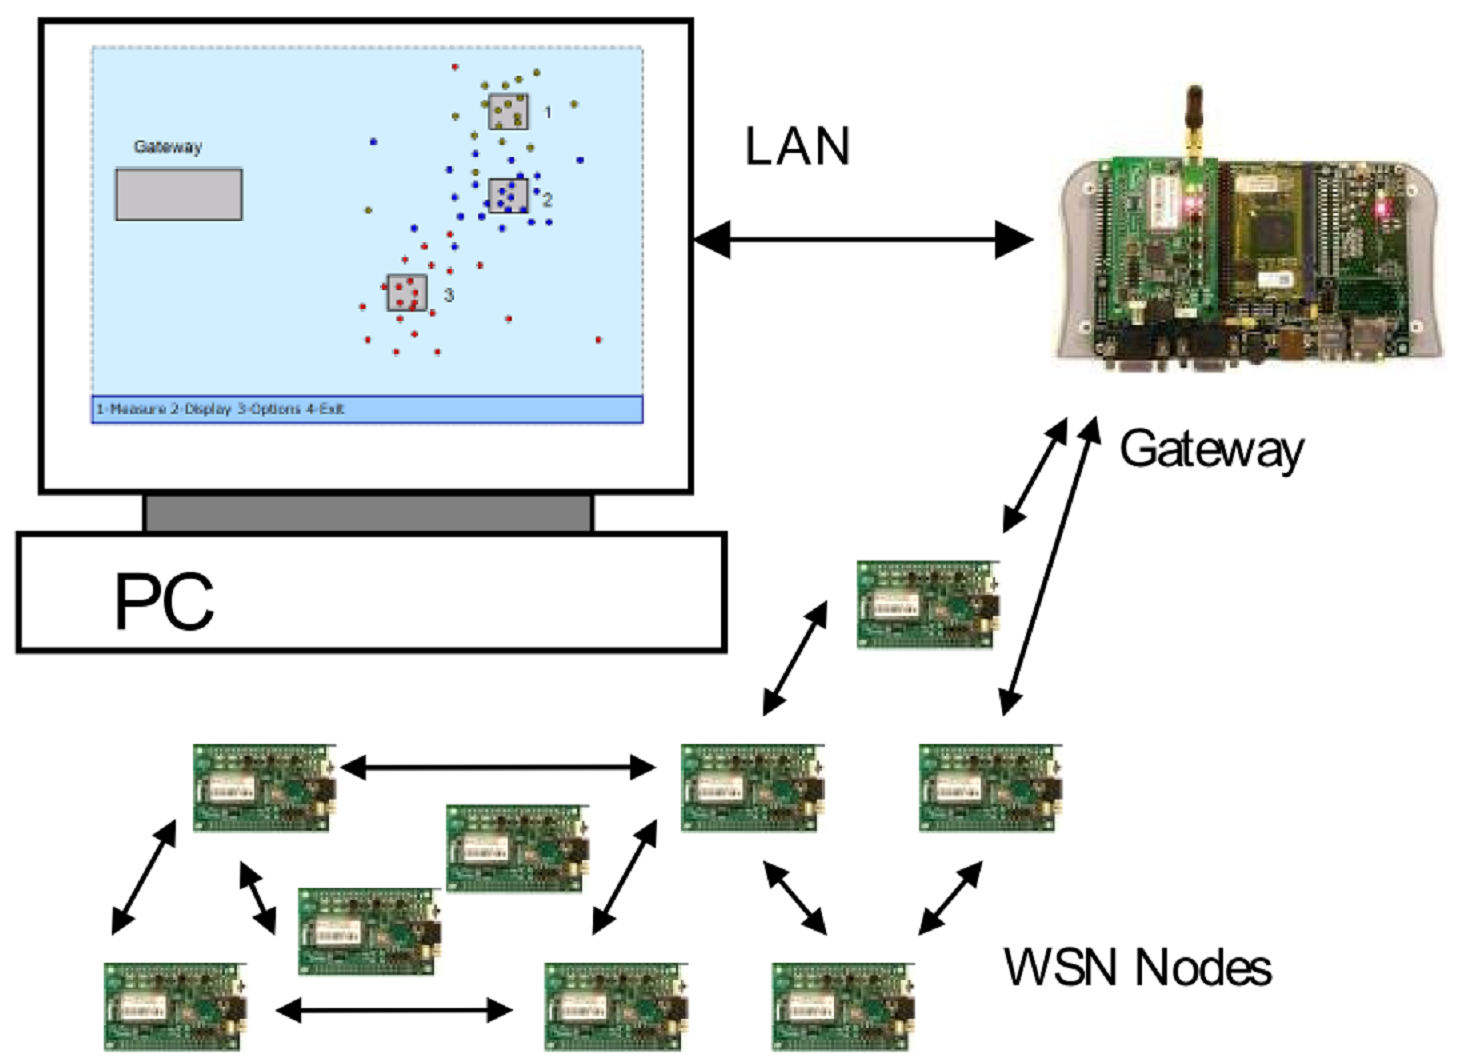
\includegraphics[width=0.82\textwidth,keepaspectration=true]{intro/overview.png}}
    \caption{Een wireless sensor network}
  \end{figure}
  \note{
    \begin{itemize}
    \item heel veel, sensoren enkele gateways
    \item netwerk bestaande uit sensoren
    \item ad-hoc netwerk technieken, geen bestaande!
    \item geen routing door 1 centrale unit
    \item communiceren via elkaar

    \end{itemize}
  }
\end{frame}

\begin{frame}{Wireless sensor networks}
  \begin{figure}
    \fbox{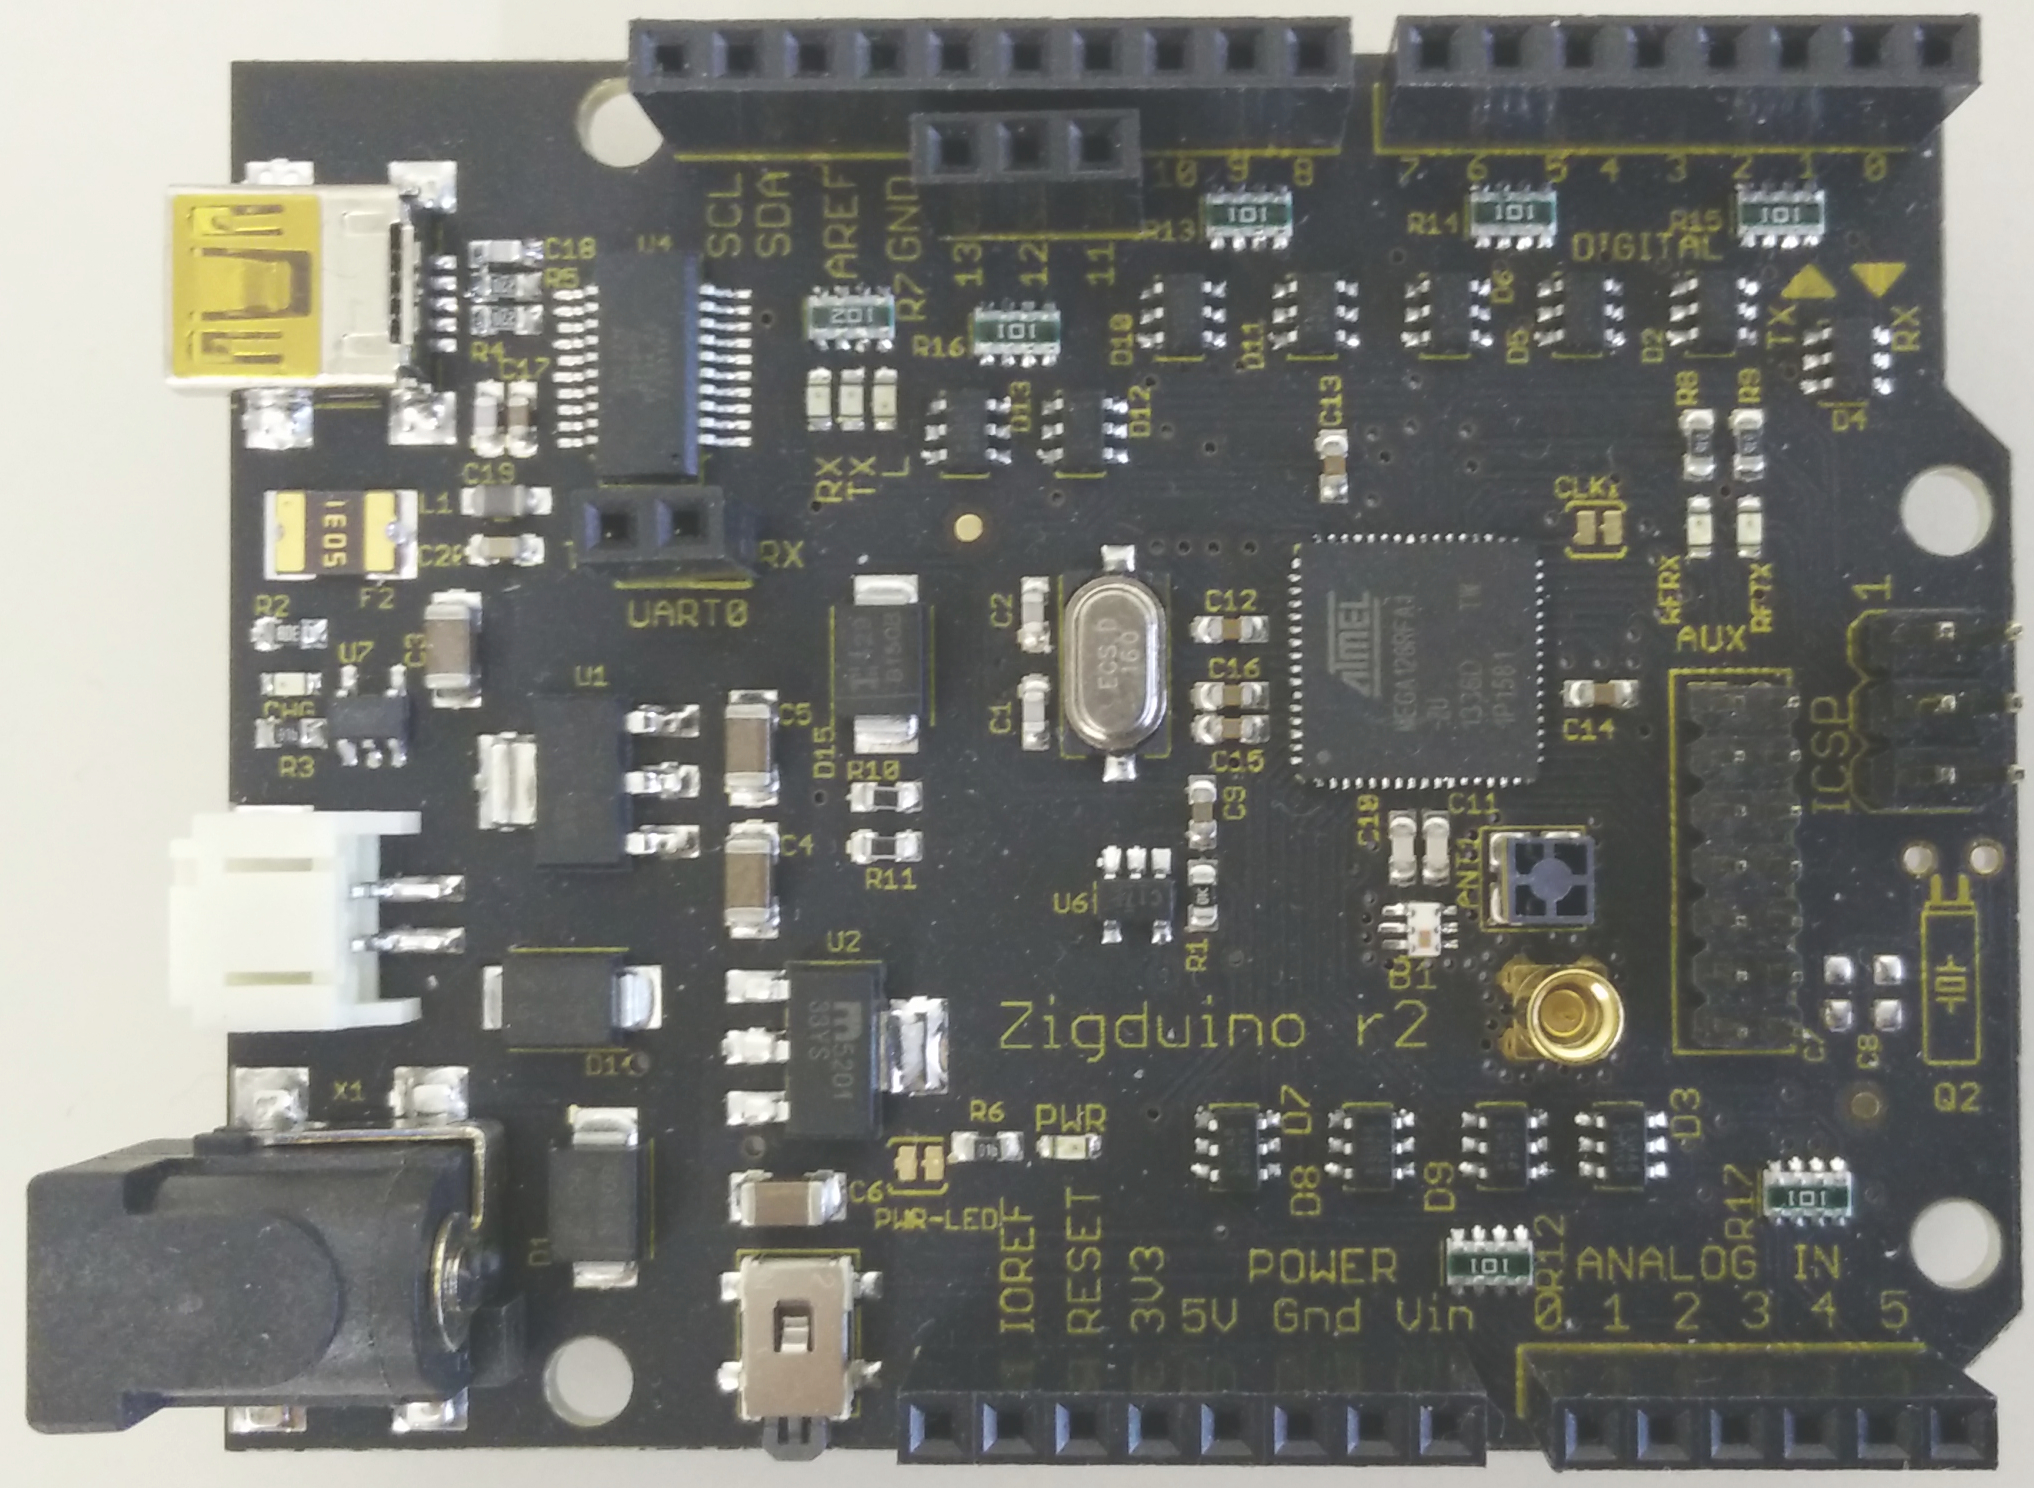
\includegraphics[height=0.78\textheight,keepaspectration=true]{zigduino.jpg}}
    \caption{Een PSUMote}
  \end{figure}
  \note{
    \begin{itemize}
    \item embedded device
    \item RF antenne, geen wifi, minder energie, groter bereik
    \item sensoren worden aangesloten
    \item microcontroller COMPUTEr ON A CHIP
    \end{itemize}
  }
\end{frame}

\begin{frame}{Wireless sensor networks}
  \begin{figure}
    \fbox{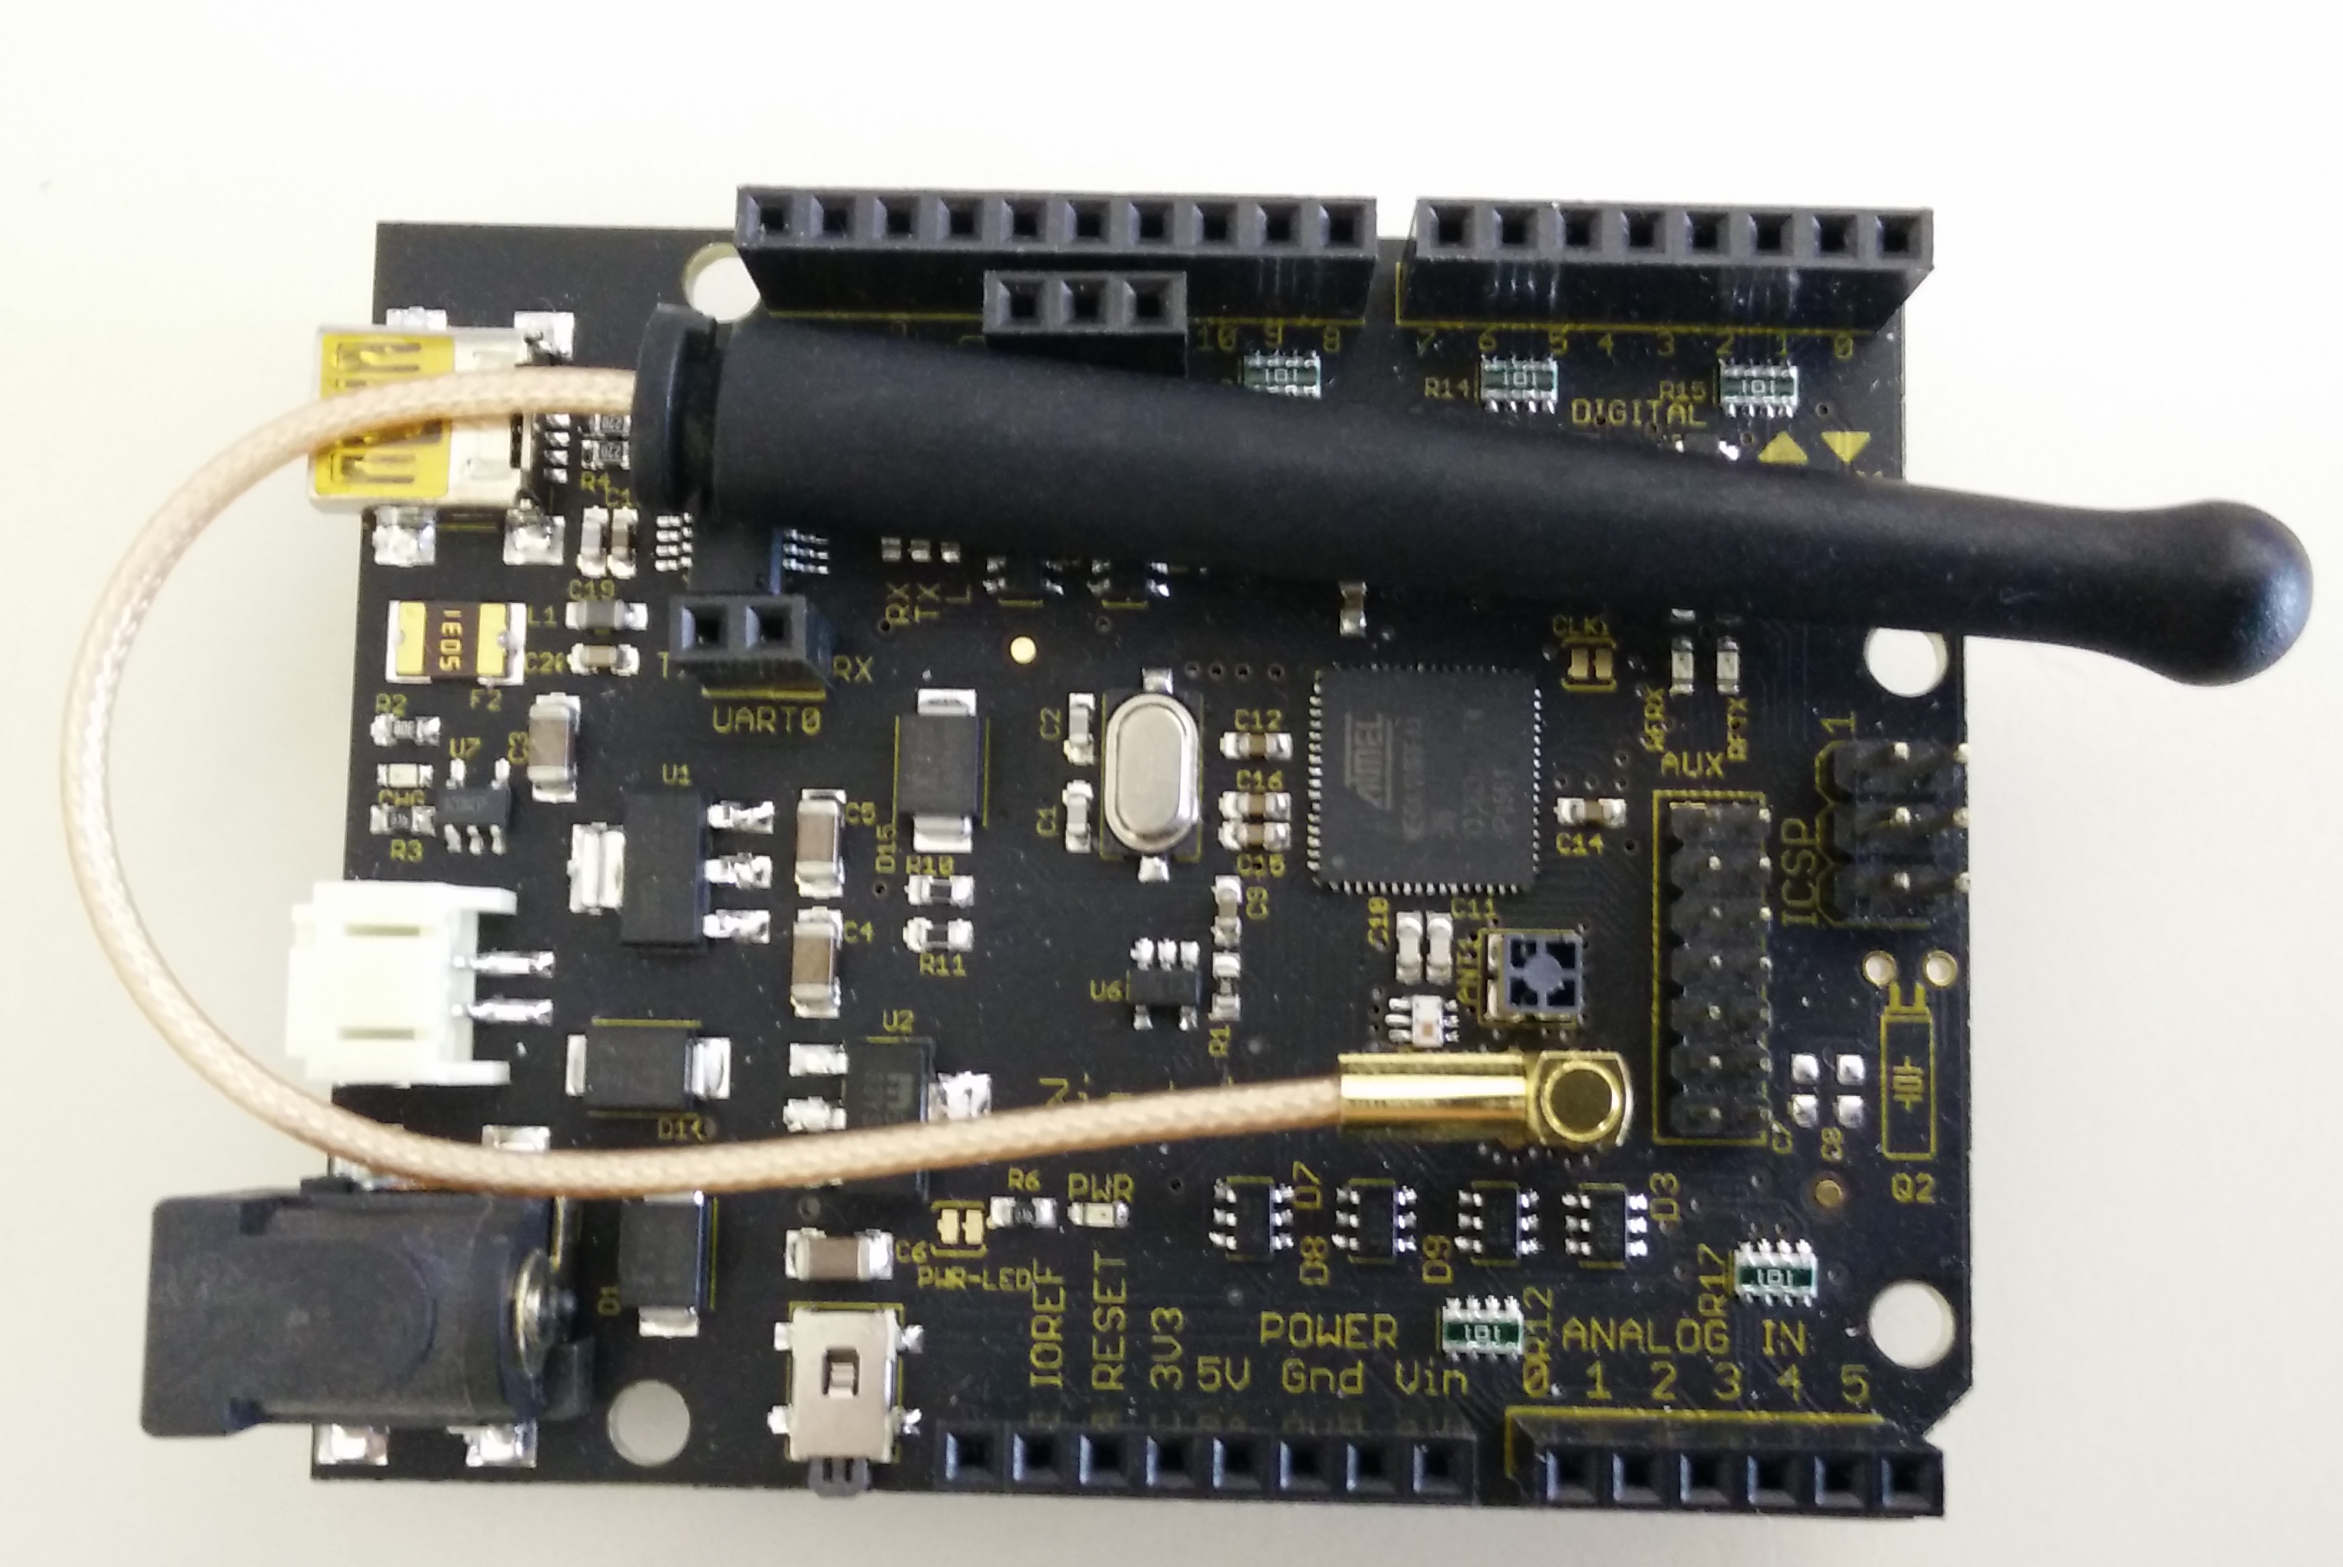
\includegraphics[height=0.78\textheight,keepaspectration=true]{zigduino_antenne.jpg}}
    \caption{Een PSUMote}
  \end{figure}
  \note{
    \begin{itemize}
    \item embedded device
    \item RF antenne, geen wifi, minder energie, groter bereik
    \item sensoren worden aangesloten
    \item microcontroller COMPUTEr ON A CHIP
    \end{itemize}
  }
\end{frame}

\begin{frame}{Belangrijke aspecten bij WSN-design}
  \uncover<2->{\begin{block}{energie-effici\"ent}
      tot 10 jaar meegaan op \'e\'en batterij
    \end{block}}%
  \uncover<3->{\begin{block}{dichtheid}
      tot 20 sensor nodes per $m^3$ (geen harde limiet)
    \end{block}}%
  \uncover<4->{\begin{block}{goedkoop}
      \$1 of minder voor heel grootschalige deployments
    \end{block}}%
  \uncover<5->{\begin{block}{autonoom}
      deploy and forget
    \end{block}}%
  \uncover<6->{\begin{block}{adaptief}
      makkelijke aanpasbare topologie, bestand tegen falen van motes
    \end{block}}
  \note{
    \begin{itemize}
    \item energie efficeit tot 10 jaar
    \item dichtheid, zie geneeskunde
    \item grote hoeveelheid, dus moet goedkoop, moet kapot gaan
    \item autonoom deploy and forget
    \item adaptief, topologie verandert, falende motes
    \end{itemize}}
\end{frame}



\section{Probleemstelling}

\begin{frame}{Probleemstelling}
\hiddencell{1}{	\large{Onze focus: \textbf{energie-efficiëntie}.}}
\hiddencell{2}{
\begin{exampleblock}{}
  {\textbf{Onderzoeksvraag:} is het energie-efficiënter om gegevens te verwerken op een embedded IoT toestel of op de back-end van het systeem?}
\end{exampleblock}}

\hiddencell{3}{
\begin{center}

\begin{tikzpicture}
\filldraw[blue_kuleuven] (0,0) -- (5,0) -- (2.5,-1) -- (0,0);
\node[text width=3cm] at (2.34,-0.25) {\textcolor{white}{Concretisering}};
\end{tikzpicture}
 
\end{center}
\begin{exampleblock}{}
  {\textbf{Onderzoeksopgave:} introduceer een simpele ?metric? om vlug te kunnen bepalen waar er bepaalde code moet uitgevoerd worden.}
\end{exampleblock}
}
\end{frame}

\section{Methodologie}
\begin{frame}{Methodologie}
\large{Energie berekenen voor:}
\vfill
\begin{tabular}{c c c}
      \hiddencell{2}{
\includegraphics[width=0.25\textwidth,keepaspectration=true]{storage}} & \hiddencell{3}{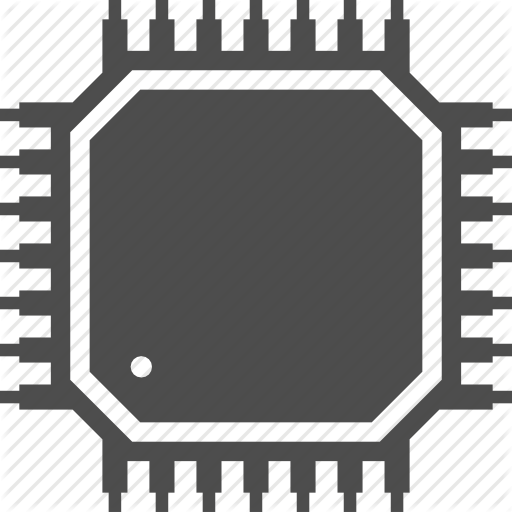
\includegraphics[width=0.25\textwidth,keepaspectration=true]{cpu}} & \hiddencell{4}{
\includegraphics[width=0.25\textwidth,keepaspectration=true]{radio}}  \\
      \hiddencell{2}{RAM-opslag} & \hiddencell{3}{berekeningen} & \hiddencell{4}{netwerkoverdracht}
    \end{tabular}
\end{frame}

\begin{frame}{Methodologie}
 
     \begin{tabular}{ p{0.3\textwidth}  p{0.6\textwidth}   }
     \toprule
      \multicolumn{1}{c}{RAM-opslag} &      \multicolumn{1}{c}{Gegevens}  \\ 
    \cmidrule(r){1-1}\cmidrule(lr){2-2}
     \raisebox{-\totalheight}{
\includegraphics[width=0.3\textwidth,keepaspectration=true]{storage}}
      & 
      \begin{itemize}
      \item \tabitem Data nog niet beschikbaar
      \hiddencell{2}{\item \tabitem Zelf experimenten uitvoeren}
      \end{itemize}
      \\ 
      
      \end{tabular}
     
\end{frame}

\begin{frame}{Methodologie}
 
     \begin{tabular}{ p{0.3\textwidth}  p{0.6\textwidth}   }
     \toprule
      \multicolumn{1}{c}{Berekeningen} &      \multicolumn{1}{c}{Gegevens}  \\ 
    \cmidrule(r){1-1}\cmidrule(lr){2-2}
     \raisebox{-\totalheight}{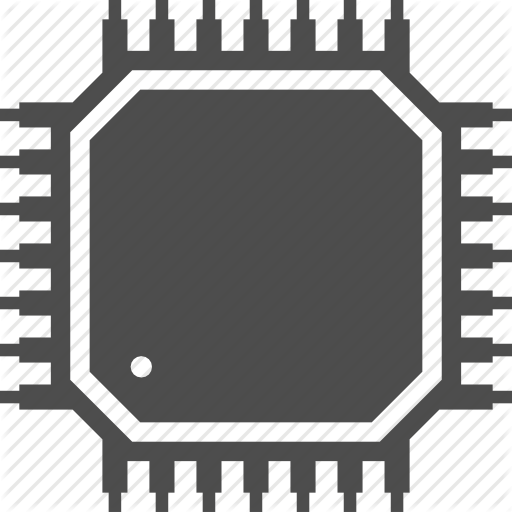
\includegraphics[width=0.3\textwidth,keepaspectration=true]{cpu}}
      & 
      \begin{itemize}
      \item \tabitem Data nog niet beschikbaar
      \hiddencell{2}{\item \tabitem Moeilijk te meten}
      \hiddencell{3}{\item \tabitem Theoretische aanpak}
      \end{itemize}
      \\ 
      
      \end{tabular}
     
\end{frame}

\begin{frame}{Methodologie}
 
     \begin{tabular}{ p{0.3\textwidth}  p{0.6\textwidth}   }
     \toprule
      \multicolumn{1}{c}{Antenne} &      \multicolumn{1}{c}{Gegevens}  \\ 
    \cmidrule(r){1-1}\cmidrule(lr){2-2}
     \raisebox{-\totalheight}
{
\includegraphics[width=0.3\textwidth,keepaspectration=true]{radio}}
      & 
      \begin{itemize}
      \item \tabitem Bestaat al deels data van
      \item \tabitem Ook moeilijk te meten
      \item \tabitem Theoretische aanpak
      \end{itemize}
      \\ 
      
      \end{tabular}
     
\end{frame}


\begin{frame}{Methodologie}
  \begin{figure}[center]
    \centering
    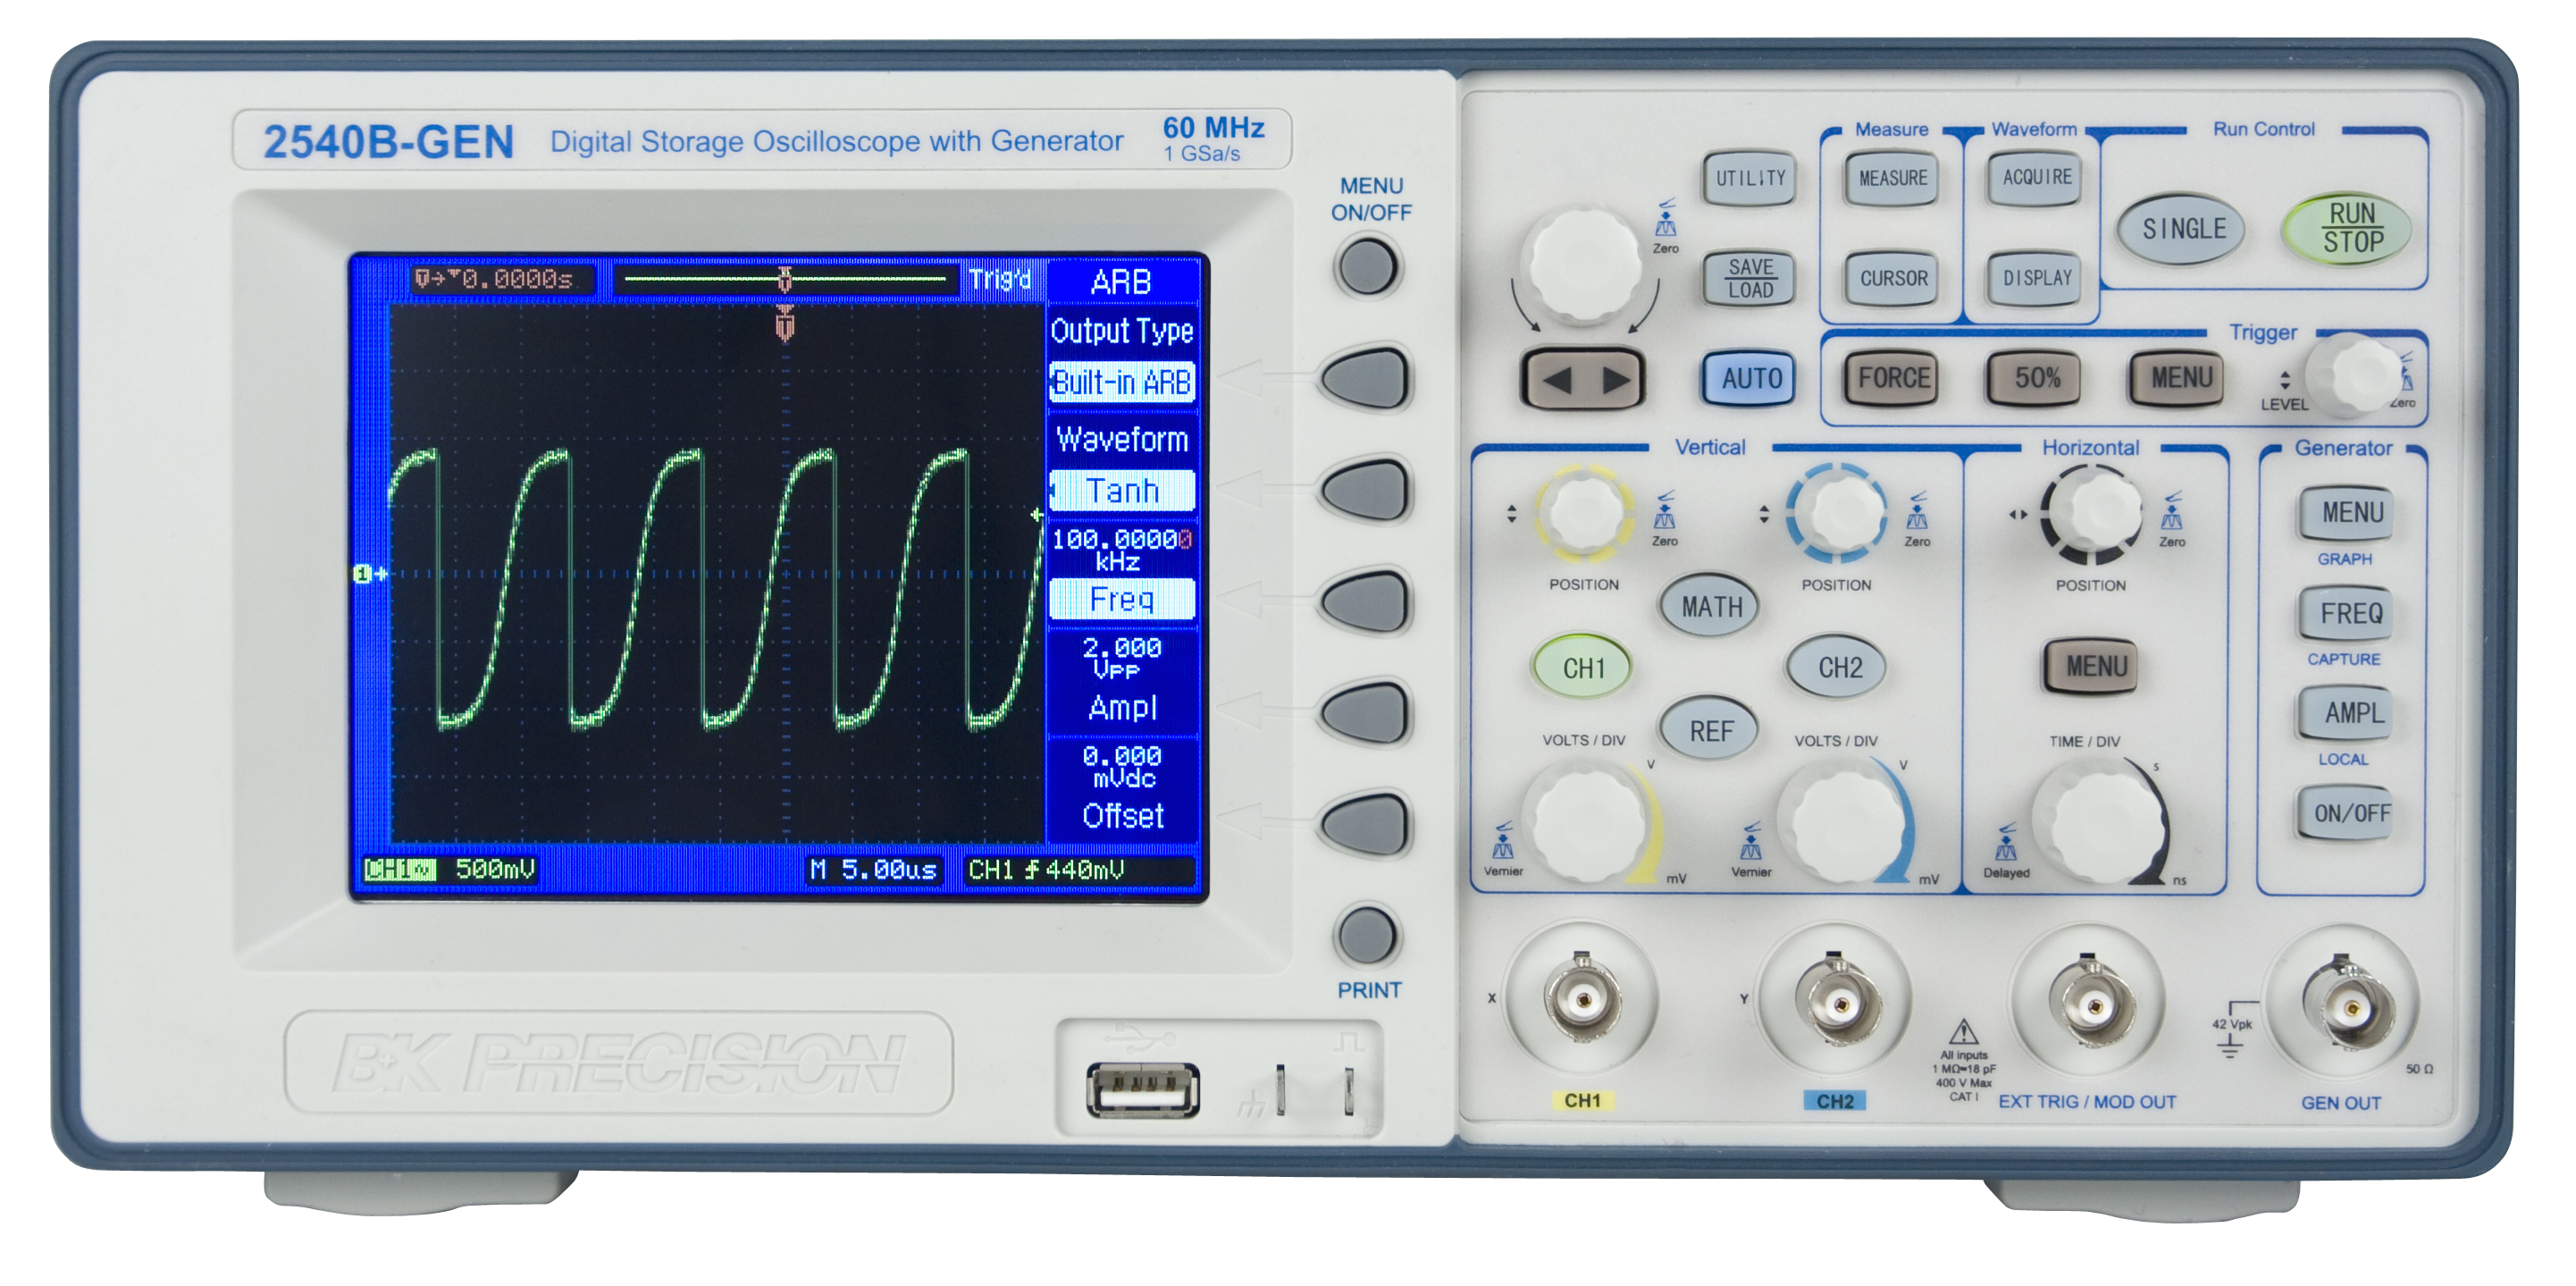
\includegraphics[width=0.9\textwidth,keepaspectration=true]{elek/dso}
    \caption{Oscilloscope}
  \end{figure}
\end{frame}

\begin{frame}{Methodologie}
  \begin{figure}[center]
    \centering
    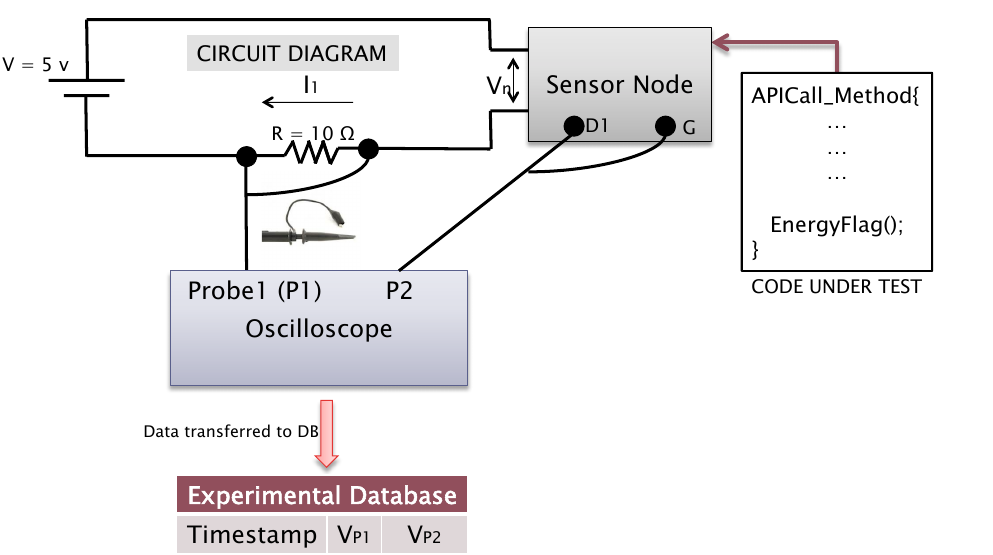
\includegraphics[width=0.9\textwidth,keepaspectration=true]{elek/diag1}
    \caption{Meetopstelling}
  \end{figure}
\end{frame}

%TODO eigen foto gebruiken!!!
\begin{frame}{Methodologie}
  \begin{figure}[center]
    \centering
    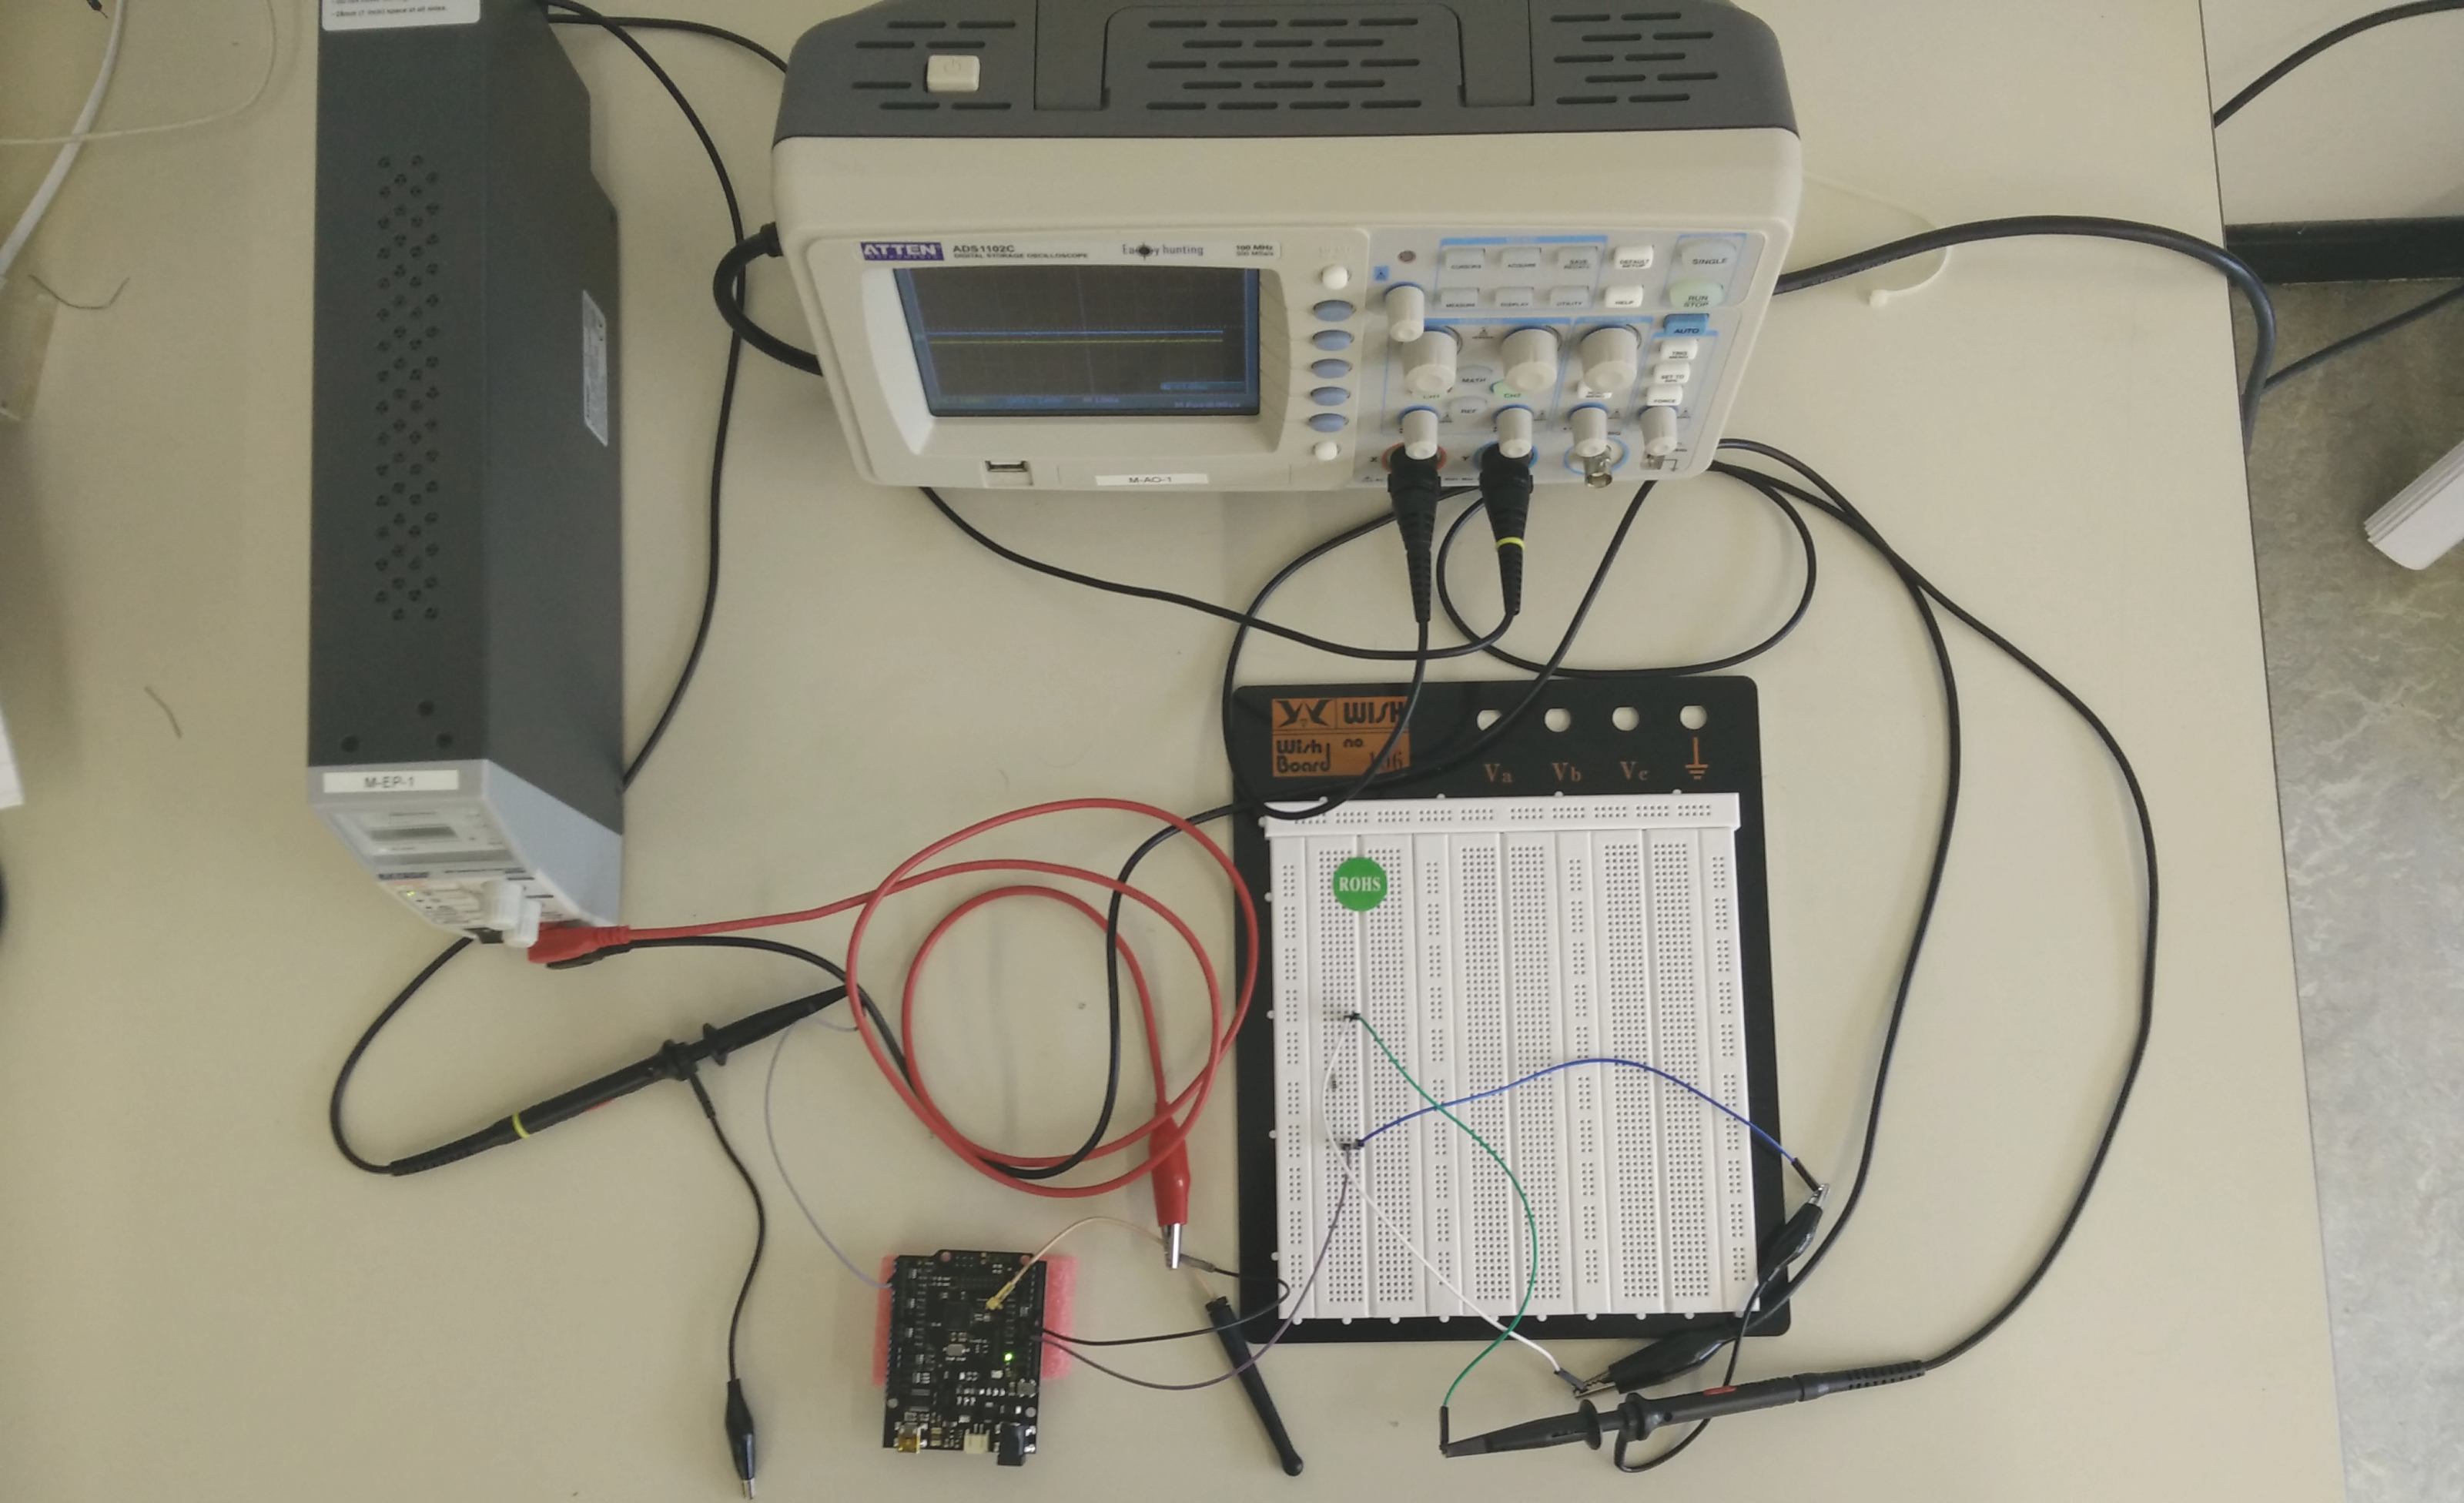
\includegraphics[width=0.9\textwidth,keepaspectration=true]{meetopstelling}
    \caption{Meetopstelling}
  \end{figure}
\end{frame}

\begin{frame}{Methodologie}
 
\begin{tabular}{ p{0.47\textwidth}  p{0.47\textwidth}   }

\begin{itemize}
      \item \textbf{1.} Maak component met triggers
      \hiddencell{2}{\item \textbf{2.} Laten uitvoeren}
      \hiddencell{3}{\item \textbf{3.} Verwerk de data}
      \end{itemize}
& 
%TODO XAVIER zorgen dat dit een mooi code voor wordt zie volgende lijn: 
%\lstinputlisting[language=C]{vbcode.c}
\\
\hiddencell{2}{
\raisebox{-\totalheight}{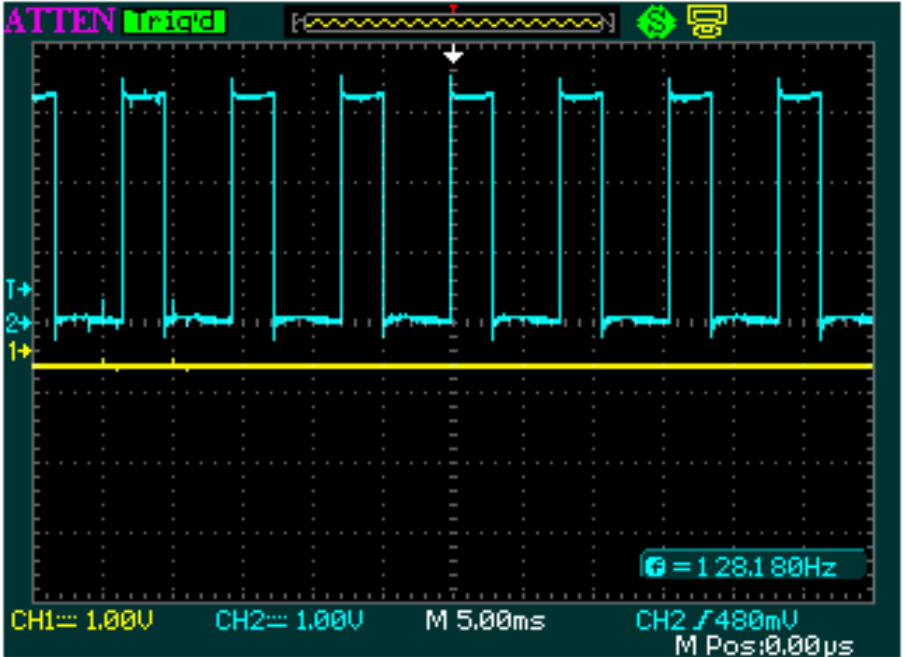
\includegraphics[width=0.4\textwidth,keepaspectration=true]{osc}}}

& 
\hiddencell{3}{
\begin{itemize} %TODO XAVIER omzetten naar verbatim
      \item Tijd[s],CH1,CH2
      \item 0.002552,-200e-3,0
      \item 0.00256,-240e-3,0
      \item 0.002568,-240e-3,3.48
      \item 0.002576,-240e-3,3.48
      \end{itemize}}
\\  
\end{tabular}    
\end{frame}
%%%%%%%%%%%%%%%%%%%%%%%%%%%%%%%%%%%%%%%%%%%%%%%%%%%%%%%%%%%%%%%%%%%%%%%%%%%%%%%%%

\begin{frame}{Methodologie}
 
     \begin{tabular}{ p{0.3\textwidth}  p{0.6\textwidth}   }
     \toprule
      \multicolumn{1}{c}{RAM-opslag} &      \multicolumn{1}{c}{Verwacht resultaat?}  \\ 
    \cmidrule(r){1-1}\cmidrule(lr){2-2}
     \raisebox{-\totalheight}{
\includegraphics[width=0.3\textwidth,keepaspectration=true]{storage}}
      & 
      \begin{itemize}
      \item \tabitem Grootte: $16kB$
      \item \tabitem Beschikbaar: $\pm 8kB$
      \item \tabitem Verwachten een lineair verband
      \item \tabitem Telkens groter aantal bytes schrijven
      \end{itemize}
      \\ 
      
      \end{tabular}
     
\end{frame}

\begin{frame}{Methodologie}
 
     \begin{tabular}{ c }
     \toprule
      \multicolumn{1}{c}{RAM-opslag}   \\ 
    \hline
     \raisebox{-\totalheight}{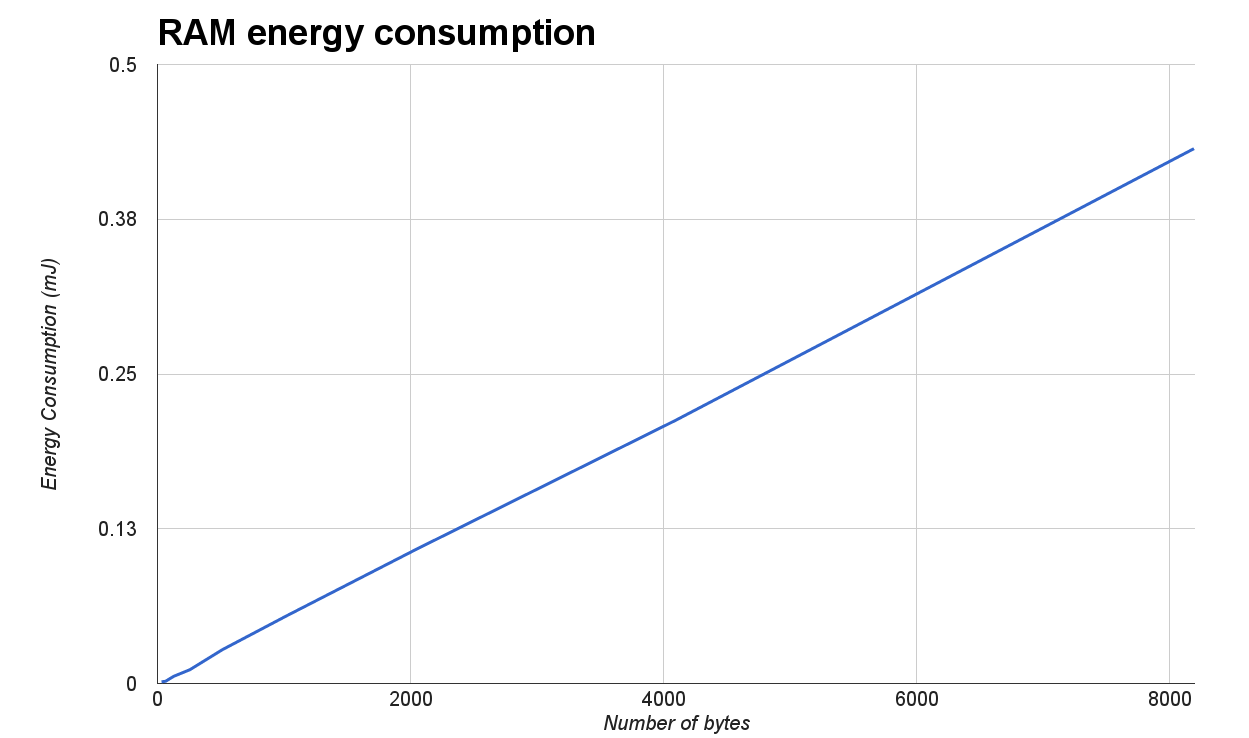
\includegraphics[width=0.95\textwidth,keepaspectration=true]{grafieken/ram_energie}}

      \\ 
      
      \end{tabular}
     
\end{frame}

\begin{frame}{Methodologie}
 
     \begin{tabular}{ p{0.25\textwidth}  p{0.7\textwidth}   }
     \toprule
      \multicolumn{1}{c}{RAM-opslag} &      \multicolumn{1}{c}{Resultaat}  \\ 
    \cmidrule(r){1-1}\cmidrule(lr){2-2}
     \raisebox{-\totalheight}{
\includegraphics[width=0.25\textwidth,keepaspectration=true]{storage}}
      & 
      \begin{itemize}
      \item \tabitem Grootte: $16kB$
      \item \tabitem Beschikbaar: $\pm 8kB$
      \item \tabitem Verwachten een lineair verband
      \item \tabitem Telkens groter aantal bytes schrijven
      \end{itemize}
      
      \framebox{\large{Lineair $\rightarrow 0.000052892mJ/Byte$}}\\
      \end{tabular}
     
\end{frame}


%%%%%%%%%%%%%%%%%%%%%%%%%%%%%%%%%%%%%%%%%%%%%%%%%%%%%%%%%%%%%%%%%%%%%%%%%%%%%%

\begin{frame}{Methodologie}
 
     \begin{tabular}{ p{0.3\textwidth}  p{0.6\textwidth}   }
     \toprule
      \multicolumn{1}{c}{berekeningen} &      \multicolumn{1}{c}{Verwacht resultaat?}  \\ 
    \cmidrule(r){1-1}\cmidrule(lr){2-2}
     \raisebox{-\totalheight}{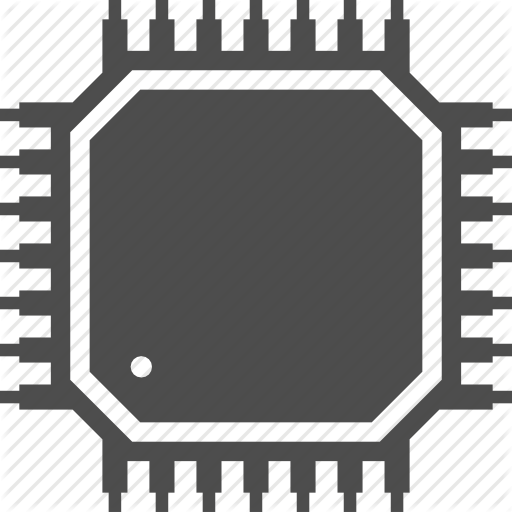
\includegraphics[width=0.3\textwidth,keepaspectration=true]{cpu}}
      & 
      \begin{itemize}
      \item \tabitem Opnieuw flags in code
      \item \tabitem Hiermee de tijd meten
      \item \tabitem Theoretische kost berekenen
      \item \tabitem Verwacht: kost verschilt van component tot component
      \end{itemize}
      \\ 
      
      \end{tabular}
     
\end{frame}

\begin{frame}{Methodologie}

     \begin{tabular}{ p{0.3\textwidth}  p{0.6\textwidth}   }
     \toprule
      \multicolumn{1}{c}{berekeningen} &      \multicolumn{1}{c}{Theretische berekening}  \\ 
    \cmidrule(r){1-1}\cmidrule(lr){2-2}
     \raisebox{-\totalheight}{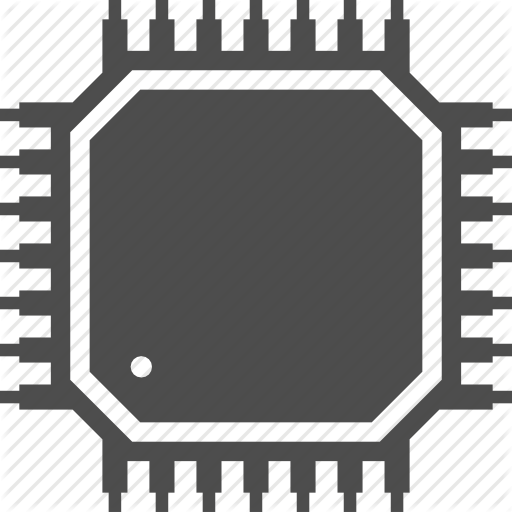
\includegraphics[width=0.3\textwidth,keepaspectration=true]{cpu}}
      & 
      \begin{itemize}
      \item \tabitem Tijd: $s$
      \item \tabitem Stroom: $3.7mA$
      \item \tabitem Voltage: $6V$
      \end{itemize}
      \framebox{Energie: $J = C \cdot V = A \cdot s \cdot V$ }
      \end{tabular}
     
\end{frame}

\begin{frame}{Methodologie}
 
     \begin{tabular}{ p{0.25\textwidth}  p{0.7\textwidth}   }
     \toprule
      \multicolumn{1}{c}{berekeningen} &      \multicolumn{1}{c}{Resultaat}  \\ 
    \cmidrule(r){1-1}\cmidrule(lr){2-2}
     \raisebox{-\totalheight}{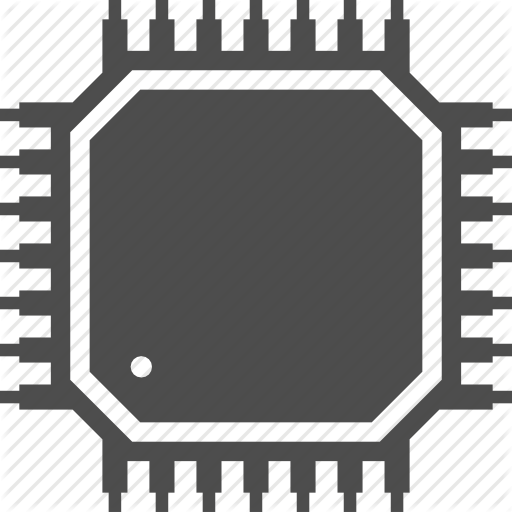
\includegraphics[width=0.25\textwidth,keepaspectration=true]{cpu}}
      & 
      \begin{itemize}
      \item \tabitem Tijd: $Ns$
      \item \tabitem Stroom: $3.7mA$
      \item \tabitem Voltage: $6V$
      \end{itemize}
      \framebox{Energie: $= 0.0037A \cdot Ns \cdot 6V$ }
      \end{tabular}
     
\end{frame}

%%%%%%%%%%%%%%%%%%%%%%%%%%%%%%%%%%%%%%%%%%%%%%%%%%%%%%%%%%%%%%%%%%%%%%%%%%%%%%%%

\begin{frame}{Methodologie}
 
     \begin{tabular}{ p{0.3\textwidth}  p{0.6\textwidth}   }
     \toprule
      \multicolumn{1}{c}{Antenne} &      \multicolumn{1}{c}{Verwacht resultaat?}  \\ 
    \cmidrule(r){1-1}\cmidrule(lr){2-2}
     \raisebox{-\totalheight}{
\includegraphics[width=0.3\textwidth,keepaspectration=true]{radio}}
      & 
      \begin{itemize}
      \item \tabitem Standaard RF-antenne
      \item \tabitem Vaste opstartkost
      \item \tabitem Daarna lineaire stijging (in functie van hoeveelheid bytes)
      \end{itemize}
      \\ 
      
      \end{tabular}
     
\end{frame}

\begin{frame}{Methodologie}
 
     \begin{tabular}{ p{0.3\textwidth}  p{0.6\textwidth}   }
     \toprule
      \multicolumn{1}{c}{Antenne} &      \multicolumn{1}{c}{Theoretische berekening}  \\ 
    \cmidrule(r){1-1}\cmidrule(lr){2-2}
     \raisebox{-\totalheight}{
\includegraphics[width=0.3\textwidth,keepaspectration=true]{radio}}
      & 
      \begin{itemize}
      \item \tabitem Tijd: $s$
      \item \tabitem Hoeveelheid bytes: $N$ 
      \item \tabitem Constante tijdskost: $113.104ms$
      \item \tabitem Tijdskost/byte: $0.382ms$
      \item \tabitem Stroom: $4.0mA$
      \item \tabitem Voltage: $6V$
      \item \tabitem $J = C \cdot V = A \cdot s \cdot V$
      \end{itemize}
        
      \end{tabular}
     \begin{center}
      \framebox{Energie $= 0.004A \cdot (N \cdot 0.382 + 113.104)ms \cdot 6V$ }      
     \end{center}
\end{frame}




\begin{frame}{Methodologie}
\begin{tabular}{ p{0.3\textwidth}  p{0.3\textwidth} p{0.3\textwidth}}
     \toprule
     & \multicolumn{1}{c}{Overzicht}  & \\ 
      \toprule
      RAM-opslag & berekeningen & Antenne\\
    \cmidrule(r){1-1}\cmidrule(lr){2-2}\cmidrule(l){3-3}
\end{tabular}      
\begin{minipage}{.33\textwidth}
      \centering
      Variabele: \# bytes\\
       \vspace{0.25cm}
      \fbox{$0.000052892mJ/Byte$} 
      
    \end{minipage}%
    \begin{minipage}{.33\textwidth}
      \centering
      Variabele N: tijdsduur\\
      \vspace{0.25cm}
      \fbox{$0.0037A \cdot Ns \cdot 6V$}
      
    \end{minipage}
     \begin{minipage}{.3\textwidth}
      \centering
      Variabele N: tijdsduur\\
      \vspace{0.35cm}
      \fbox{\parbox{\textwidth}{$0.004A \cdot (N \cdot 0.382$ \\ $+ 113.104)ms \cdot 6V$}}
     
    \end{minipage}
\end{frame}
%%%%%%%%%%%%%%%%%%%%%%%%%%%%%%%%%%%%%%%%%%%%%%%%%%%%%%%%%%%%%%%%%%%%%%%%%%%%%%%%
%%%%%%%%%%%%%%%%%%%%%%%%%%%%%%%%%%%%%%%%%%%%%%%%%%%%%%%%%%%%%%%%%%%%%%%%%%%%%%%%
%%%%%%%%%%%%%%%%%%%%%%%%%%%%%%%%%%%%%%%%%%%%%%%%%%%%%%%%%%%%%%%%%%%%%%%%%%%%%%%%
%%%%%%%%%%%%%%%%%%%%%%%%%%%%%%%%%%%%%%%%%%%%%%%%%%%%%%%%%%%%%%%%%%%%%%%%%%%%%%%%
%%%%%%%%%%%%%%%%%%%%%%%%%%%%%%%%%%%%%%%%%%%%%%%%%%%%%%%%%%%%%%%%%%%%%%%%%%%%%%%%
%%%%%%%%%%%%%%%%%%%%%%%%%%%%%%%%%%%%%%%%%%%%%%%%%%%%%%%%%%%%%%%%%%%%%%%%%%%%%%%%
%%%%%%%%%%%%%%%%%%%%%%%%%%%%%%%%%%%%%%%%%%%%%%%%%%%%%%%%%%%%%%%%%%%%%%%%%%%%%%%%
%%%%%%%%%%%%%%%%%%%%%%%%%%%%%%%%%%%%%%%%%%%%%%%%%%%%%%%%%%%%%%%%%%%%%%%%%%%%%%%%
\section{Voorgestelde oplossing}

\begin{frame}{Voorgestelde oplossing}
%TODO XAVIER: onze metric in een mooie formule gieten
\end{frame}

\section{Resultaten}
\begin{frame}{Resultaten}

\end{frame}


\section{Conclusie \& verder werk}
\begin{frame}{Conclusie}
Voor of na verder werk laten komen?
\end{frame}

\begin{frame}{Verder werk}
\end{frame}

%%%%%%%%%%%%%%%%%%%%%%%%%%%%%%%%%%%%%%%%%%%%%%%%%%%%%%%%%%%%%%%
\begin{frame}[allowframebreaks]{Bibliografie}

%  \addtocategory{papers}{akyildiz2002wireless}
%  \addtocategory{papers}{mainwaring2002wireless}
%  \addtocategory{papers}{hughes2009looci}
%  \addtocategory{papers}{hughes2013energy}
  \nocite{*}
%  \textbf{Papers}
%  \printbibliography[category=papers]
%  \newpage
%  \textbf{Afbeeldingen}
%  \printbibliography[type=misc]
  \printbibliography
\end{frame}

\end{document}